\documentclass[11pt,a4paper,english]{article}
\usepackage[left=2.4cm,right=2.4cm,top=2.4cm,bottom=2.4cm]{geometry}
\usepackage{helvet}

\usepackage[authoryear]{natbib}
\usepackage{color}
\definecolor{Gray}{gray}{.25}
\usepackage{url}
\usepackage{amsmath}
\usepackage{graphicx}


% production makros
\usepackage{todonotes}
\newcommand{\TODO}[1]{\begingroup\color{red}#1\endgroup}
\newcommand{\raim}[1]{\begingroup\color{blue}#1\endgroup}
\usepackage[normalem]{ulem}

% useful text makros
% strains
\newcommand{\ifo}{IFO~0233}

\usepackage[load=abbr, separate-uncertainty=true, multi-part-units=single]{siunitx}
%\DeclareSIUnit{\Molar}{\textsc{M}} % pg. 39 siunitx manual (2013/03/11)
% old version of siunitx doesnt speek above
\newcommand{\Mol}{\textsc{M}}%\mole\per\litre}
\newcommand{\mM}{\milli\textsc{M}}%\mole\per\litre}
\newcommand{\uM}{\micro\textsc{M}}%\mole\per\litre}
\newcommand{\nM}{\nano\textsc{M}}%\mole\per\litre}
%\newcommand{\cmol}{C-\mol}%\mole\per\litre}
%\DeclareSIUnit{\cmol}{C-mol}
\newcommand{\cmol}{\textsc{C-}\si{\mole}}
\newcommand{\cmmol}{\textsc{C-}\si{\milli\mole}}

%% elements and molecules 
\newcommand{\ox}{\ensuremath{\text{O$_2$}}}
\newcommand{\cox}{\ensuremath{\text{CO$_2$}}}
\newcommand{\hs}{\ensuremath{\text{H$_2$S}}}
\newcommand{\elec}{\ensuremath{\text{e}^-}}
\newcommand{\prot}{\ensuremath{\text{H}^+}}
\newcommand{\pH}{\ensuremath{\text{pH}}} 

%% specific fluxes
\newcommand{\qatp}{\ensuremath{q_\text{ATP}}}
\newcommand{\qh}{\ensuremath{q_\text{H$^+$}}}
\newcommand{\qoh}{\ensuremath{q_\text{OH$^-$}}}
\newcommand{\qox}{\ensuremath{q_\text{O$_2$}}}
\newcommand{\qcox}{\ensuremath{q_\text{CO$_2$}}}
\newcommand{\RQ}{\ensuremath{\text{RQ}}}
%% total culture fluxes 
\newcommand{\ratp}{\ensuremath{r_\text{ATP}}}
\newcommand{\rh}{\ensuremath{r_\text{H$^+$}}}
\newcommand{\roh}{\ensuremath{r_\text{OH$^-$}}}
\newcommand{\rox}{\ensuremath{r_\text{O$_2$}}}
\newcommand{\rcox}{\ensuremath{r_\text{CO$_2$}}}


%% yields
\newcommand{\por}{\ensuremath{P_\text{O}}}
\newcommand{\per}{\ensuremath{P_\text{2\elec}}}
\newcommand{\phr}{\ensuremath{P_\text{\prot}}}
\newcommand{\yatp}{\ensuremath{y_\text{ATP}}}

%% some useful tex makros
\newcommand{\etal}[0]{\textit{et al.}}
\newcommand{\ie}[0]{\textit{i.e.}}
\newcommand{\eg}[0]{\textit{e.g.}}
\newcommand{\vs}[0]{\textit{vs.}}
\newcommand{\cf}[0]{\textit{cf.}}
\newcommand{\via}[0]{\textit{via}}
\newcommand{\invivo}[0]{\textit{in~vivo}}
\newcommand{\invitro}[0]{\textit{in~vivo}}

\newcommand{\tmin}{\ensuremath{T_\text{min}}}
\newcommand{\tmax}{\ensuremath{T_\text{max}}}
\newcommand{\tpar}{\ensuremath{T_\text{P}}}
\newcommand{\toff}{\ensuremath{T_\text{O}}}
\newcommand{\tosc}{\ensuremath{T_\text{osc}}}
\newcommand{\thoc}{\ensuremath{T_\text{hoc}}}
\newcommand{\tloc}{\ensuremath{T_\text{loc}}}
\newcommand{\phoc}{\ensuremath{\phi_\text{hoc}}}
\newcommand{\fmin}{\ensuremath{f_\text{min}}}
\newcommand{\fmax}{\ensuremath{f_\text{max}}}
\newcommand{\fosc}{\ensuremath{f_\text{osc}}}

\setlength{\parindent}{0em}
\setlength{\parskip}{1ex}

\let\cite\citep

\title{Finding \ifo{}: History of a Peculiar Strain from the Japenese Culture Collection}
\author{Louis Goldschmidt, Nikolaus Thumm, Rainer Machn{\'e}}

\begin{document}

\maketitle

\section{Introduction}
In 1992, Kuriyama's lab first reported stable oscillations of
respiratory activity in continuous cultures of the
\textit{Saccharomyces cerevisiae} strain \ifo{}
\cite{Satroutdinov1992, Keulers1996a, Keulers1996b}. The data, online
recording of dissolved oxygen concentration (DO) in the culture,
looked similar to a well known phenomenon from budding yeast
continuous culture: when grown at low dilution rates and high cell
density, cells tend to synchronize their cell division cycle (CDC)
\cite{Finn1954, vonMeyenburg1969, Kuenzi1969, Muench1992}. The period
of this type of oscillation is shorter than the average culture
doubling time, which, at stable biomass, is set by the continuous
culture dilution rate \cite{Bellgardt1994a, Bellgardt1994b,
  Hjortso1995, Duboc2000}.  Since slowly growing yeast produce smaller
daughter cells, these take longer to divide, and theoretical models
assumed that the observed period of metabolic dynamics correspond to
the division time of the larger mother cells. Daugther cells would
spend a one or more of those cycles with cell growth in G1 phase
before they can become mother cells themselves.

But the oscillations of the \ifo{} cultures had periods of
\SIrange{40}{60}{\min}, at average culture doubling time of
\SIrange{6}{12}{\hour}. This was too fast for partial synchronization
of the CDC and could thus not be easily explained by the existing
models. It was also too slow for so-called glycolytic oscillations,
with periods of only a few minutes \citep{Ghosh1964}.  The closest
observations was that of Mochan and Pye \cite{Mochan1973} who observed
a series of high amplitude oscillations of DO, in batch culture on
glucose medium and after the diauxic switch, when cells start to
consume the ethanol produced in the batch phase. Here, periods ranged
from \SIrange{30}{90}{\min} and varied between experiments. These
phenomena thus pointed to a more fundamental tendency of the
metabolism to show periodic behaviour, independent of the CDC
\cite{Aon2008, ONeill2020, Machne2021pre}.

Meanwhile a wealth of transcriptome and physiological data has been
collected on both, the short period oscillation of \ifo{}, as well as
long period and CDC-coupled systems. In both systems, DNA synthesis
(S-phase) is initiated preferentially at the time of maximal
respiratory activity \cite{klevecz04, Slavov2011, Burnetti2016}.
Independent of the period, a conserved temporal transcription program
procedes from expression of cell growth-related genes (ribosomal RNA
processing, ribosomal proteins), to biosynthetic genes (amino acid
synthesis), mitochondrial genes (tricarboxylic acid cycle, electron
transport genes, and mitochondrial ribosomal proteins), to a large
gene group that comprises of sugar, lipid and protein catabolic genes,
and genes expressed as a response to all kind of stress conditions
\cite{Machne2012, Machne2017phd, Machne2021pre}. Periods appear
strain-specific, and it was suggested that the observed periods are
related to the strain-specific growth rate at which cells start to
additionally ferment glucose instead of relying exclusively on
respiratory metabolism \cite{Burnetti2016, Machne2017phd}.
Fermentation set in at growth rates of about \SI{0.11}{\per\hour} in
\ifo{} \cite{Satroutdinov1992}, while other strains grow exclusively
with respiratory metabolism at growth rates up to
\SIrange{0.2}{0.3}{\per\hour}. Relating observed periods to
this critical growth rate indicates that the two phenomena may
be related (Fig.~), and cells would show a minimal period of
about \SI{30}{\min} when growing at this rate. However, these
observations are purely phenomenological, and the causes
and consequences of respiratory metabolism remain largely elusive.

Here we attempt to gather further information on the identity of this
strain, which allowed to collect interesting further information on
the source and phenotypic properties of this strain.

\section{Results}

\subsection{Tracing \ifo{} to an Old German Distillery Strain}
The strain identifier \ifo{} is from the Japanese
culture collection NBRC and therein it is annotated as \texttt{Application:
  Distillery yeast Rasse II}, ``accepted'' in 1941, and as ``ATCC~560'' in
the US American culture collection. The ATCC entry further specifies
the strain history as \texttt{ATCC <<--Wallerstein Co.,
  Inc.<<--Inst. Garungsgewerbe, Race II}.  A ``Wallerstein Company,
Inc.''  was a consultation, research and production company in
fermentation and enzyme technology in New York, founded by the
brothers Max (c.1875-1937) and Leo (c.1882-1958) Wallerstein,
Jewish-German emigrants from Fuerth in
Bavaria \footnote{\url{https://collection.cooperhewitt.org/people/18052753/bio},\\ \url{https://www.sciencephoto.com/media/621983/view/leo-wallerstein-german-us-chemist}}
The ``Brennereihefe, Rasse II'' can be further traced to a strain
isolated as ``Hefe 128'' by Paul Lindner in 1889 from samples of a
distillery in Gronowo (West Prussia, now Poland) which obtained their
yeast from a dry yeast supplier in the city Thorn (now Toru\'n,
Poland) \cite{Lindner1895}. At the Berlin Institut f\"ur
G\"arungsgewerbe (now with the addition ``und Biotechnologie'',
\url{www.ifgb.de}), Lindner and Max Delbr\"uck (the uncle) had
established axenic cultures of many yeasts (\textit{Reinzuchthefe}),
and ``Hefe 128'' became ``Brennereihefe, Rasse II'', a commercially
successful and intensively studied strain at the time
\cite{Lindner1895, Lindner1919}. In 1908 ``Rasse XII'' had apparently
won the commercial race in distilleries \cite{Kohl1908}.  The
``accepted'' date at NBRC, 1941, makes it likely that, due to
alliances in World War II, the Japenese collection had obtained a
sample directly from Berlin. The exact relation of \ifo{} to ATCC~560
and ``Hefe 128'' remains to be established.

``Hefe 128'' formed regular concentric ring structures in colonies
(Fig. \ref{fig:hefe128}A) \cite{Lindner1895}, had high alcohol tolerance, and
its use in industrial context, \eg{}, tested in 181 distilleries by
surveys \cite{Dingler1894}, increased the alcohol yield but caused
excessive foaming \cite{Behrend1900}. As a fermentation yeast
(\textit{G\"arhefe}), it outgrowed \textit{Wuchshefe} (``growth
yeast'') only at low aeration of the culture \cite{Haehn1952}.
%
In micrographs of a foaming potato mash (\ref{fig:hefe128}B)
\cite{Lindner1903}, and again in later studies on minimal (``mineral'')
media (in search of Wildiers ``Bios'', now known as biotin), a
researcher named Chrzaszgz observed large cells, with granulated
cytoplasm and large lipid inclusions \cite{Lindner1919}.
%
%... intensively studied in pre-WWI Germany,
%\eg{}, surveys were sent to 181 distilleries
%, where all could increase ethanol yield but
%many reported significant foaming problems, \cite{Dingler1894}
%and usied
%
\subsection{Isolated Descriptions in Modern Literature}

Until Kuriyama's studies the strains deposited in culture collections
were rarely used, although searches for alternative designations as
``\textit{S. cer.} var. \textit{ellipsoides}'', ``\textit{S. cer.}
Hansen'' or ``\textit{Candida robusta} Diddens \& Lodder'', or its ID in
other culture collections (CBS 6140, NBRC 2058, NRRL Y-635) may yield
further results. Especially the Russian culture collection (XYZ)
appears to house several ``Rasse'' strains from Lindner's collection
\cite{Naumova2013}.

ATCC~560 was transformable \cite{Casey1988}, as was
\ifo{} \cite{Adams2003} and had a ``normal'' karyotype and only one
allele of ILV2 \cite{Casey1988b}. It had sparked short interest for
expressing catalase and superoxide dismutase \cite{Gregory1974}, and
was characterized as an ``early'' fermenter in continuous culture
where fermentation set in at a low dilution (growth) rates between
0.1\si{\per\hour} and 0.15\si{\per\hour} \cite{Hansson1983},
consistent with the value 0.11\si{\per\hour} reported for \ifo{}
\cite{Satroutdinov1992} and its initial isolation as a distillery
yeast.

\begin{figure}[ht] 
  \centering
  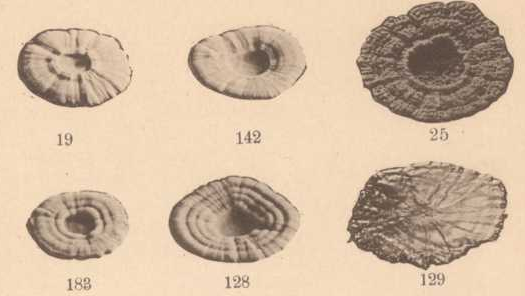
\includegraphics[width=.4\linewidth]{figures/lindner1895_TafelII_top.png}
  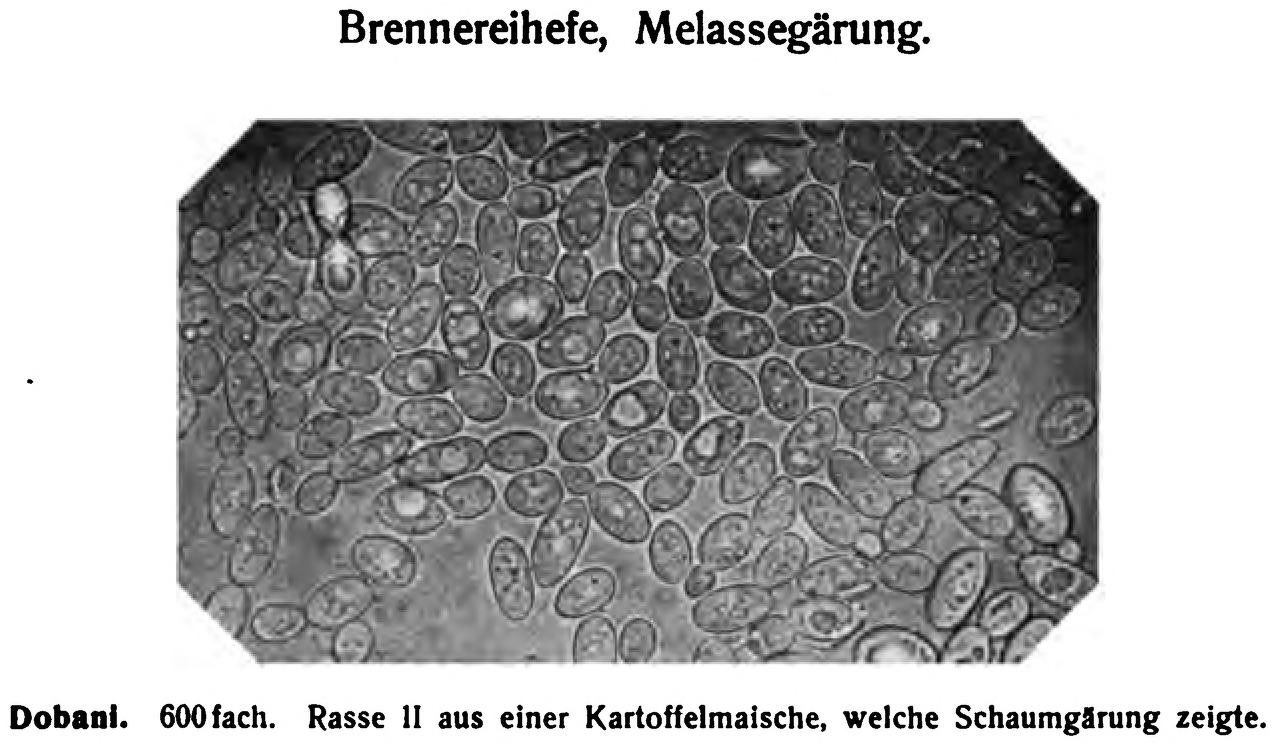
\includegraphics[width=.49\linewidth]{figures/lindner03_tafel56_top.png}\\
  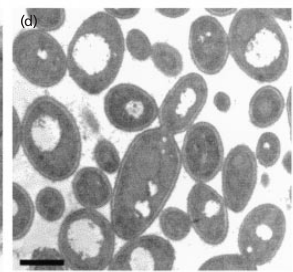
\includegraphics[width=.35\linewidth]{figures/lloyd02_fig6d.png}
  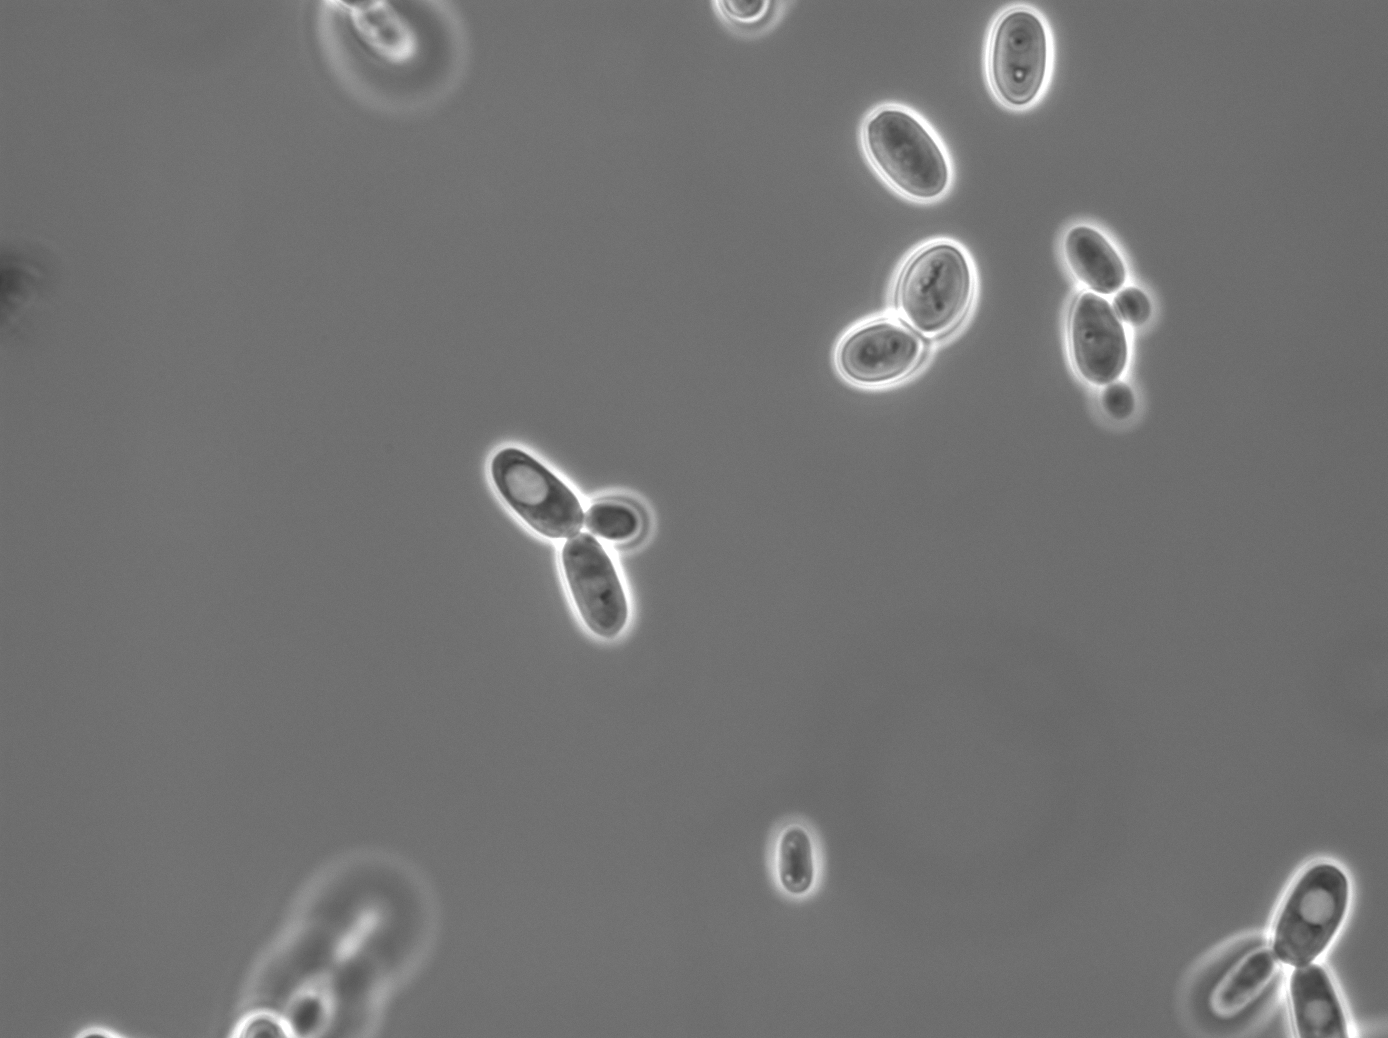
\includegraphics[width=.45\linewidth]{figures/Aufnahme-24.png}

  \caption{\textbf{Historical Records.}  A: a colony of the isolated
    strain ``Hefe 128'' shows regular concentric rings (grown on 6\%
    \textit{W\"urzgelatine}), reproduced from ``Tafel II'' of
    \citet{Lindner1895}.  B: ``Hefe 128'' later became
    ``Brennereihefe, Rasse II'' and shows large granulated cells with
    oil drops in likely ``stressed'' conditions, here seen in
    micrographs from a foam-building fermentation of potato mash
    (reproduced from ``Tafel 56'' in \citet{Lindner1903}). (via the
    \texttt{archive} project, and an online word doc; permission,
    correct citation). C: electronmicroscopy of \ifo{} by
    \citet{Lloyd2002b}.  D: ``Rasse II'' survived in the freezers of
    the Berlin Institut f\"ur G\"arungsgewerbe und
    Biotechnologie''. Micrographs from 2020-01-22.}
  \label{fig:hefe128}
\end{figure}

\subsection{The Scottish Whiskey ``Strain M''?}

blog entry

\subsection{Reviving Rasse II}

show growth in calorimeter, no oscis, bad mixing?

\section{Discussion}

1941: war-relevant for biofuel production?

short period and low dilution rate Dcrit

concentric rings and short-period oscillations?

lipid inclusions: lipids instead of glycogen?

final answer requires genome sequencing, but meanwhile
IFO: identified fungal object

\bibliographystyle{apalike}

%% and use `bibexport -o strain_history.bib strain_history.aux` to update local
\bibliography{strain_history}
%\bibliography{/home/raim/ref/tata}

\end{document}
